\documentclass[a4paper]{article}

\usepackage{INTERSPEECH2018}
\usepackage{multirow}
% \usepackage{tipa}
\usepackage{amsmath}
\usepackage{booktabs}
\usepackage{url}
\usepackage{cite}
\usepackage{epstopdf}
\newcommand{\quotes}[1]{``#1''}
\setlength{\intextsep}{10pt plus 2pt minus 3pt} %distance between floats on the top or the bottom and the text
\setlength{\textfloatsep}{14pt plus 0pt minus 4pt}%distance between two floats
\setlength{\floatsep}{12pt plus 0pt minus 2pt}%distance
% \newcommand{\etal}{\textit{et al}.~}
% \setlength{\intextsep}{10pt plus 1pt minus 3pt} %distance between floats on the top or the bottom and the text
% \setlength{\textfloatsep}{14pt plus 0pt minus 4pt}%distance between two floats
% \setlength{\floatsep}{12pt plus 0pt minus 2pt}%
% \title{Multilingual TDNN-BLSTM Acoustic Model with Language-Dependent Pre-Final Layers for Improved ASR}
\title{Improving Cross-Lingual Knowledge Transferability Using Multilingual TDNN-BLSTM with Language-Dependent Pre-Final Layer}
\name{Siyuan Feng, Tan Lee}
% \name{Siyuan Feng, Tan Lee\thanks{We thank Yuzhong Wu for RASC-863 dataset processing work. This research is partially supported by a GRF project grant (Ref: CUHK 14227216) from Hong Kong Research Grants Council.}}
\address{
  Deparment of Electronic Engineering, The Chinese University of Hong Kong, Hong Kong}
\email{siyuanfeng@link.cuhk.edu.hk, tanlee@ee.cuhk.edu.hk}

\begin{document}

\maketitle
%
\begin{abstract}
Multilingual acoustic modeling for improved automatic speech recognition (ASR) has been extensively researched. It's widely acknowledged that the shared-hidden-layer multilingual deep neural network (SHL-MDNN) acoustic model (AM) could outperform the conventional monolingual AM, due to its effectiveness in cross-lingual knowledge transfer. In this work, two research aspects are investigated, with the goal of improving multilingual acoustic modeling. Firstly, in the  SHL-MDNN architecture, the shared hidden layer configuration is replaced by a combined TDNN-BLSTM structure. Secondly, the improvement of cross-lingual knowledge transferability is achieved through adding the proposed language-dependent pre-final layer under each network output. The pre-final layer, rarely adopted in past works, is expected to increase nonlinear modeling capability between universal transformed features generated by shared hidden layers and language-specific outputs. Experiments are carried out with CUSENT, WSJ and RASC-863 corpora, covering Cantonese, English and Mandarin. A Cantonese ASR task is chosen for evaluation. Experimental results show that SHL-MTDNN-BLSTM achieves the best performance. The proposed additional language-dependent pre-final layer brings moderate while consistent performance gains in various multilingual training corpora settings, thus demonstrates its effectiveness in improving cross-lingual knowledge transferability.
  % For your paper to be published in the conference proceedings, you must use this document as both an instructiyou will be asked to fix it.

  % Please do not reuse your past papers as a template. To prepare your paper for submission, please always download a fresh copy of this template from the conference website and please read the format instructions in this template before you use it for your paper.
  % Conversion to PDF may cause problems in the resulting PDF or expose problems in your source document. Before submitting your final paper in PDF, check that the format in your paper PDF conforms to this template. Specifically, check the appearance of the title and author block, the appearance of section headings, document margins, column width, column spacing, and other features such as figure numbers, table numbers and equation number. In summary, you must proofread your final paper in PDF before submission.
    % The maximum number of pages is 5. The 5\textsuperscript{th} page may be used exclusively for references. The references should begin on an earlier page immediately after the Acknowledgements section, and continue onto the 5\textsuperscript{th} page. If no space is available on an earlier page, then the references may begin on the 5\textsuperscript{th} page.

  % Index terms should be included as shown below.
\end{abstract}
\noindent\textbf{Index Terms}: multilingual acoustic model, TDNN, BLSTM, cross-lingual knowledge transfer

\section{Introduction}
\label{Intro}
In recent years there has been a significant research interest in developing technologies for multilingual speech modeling, especially in the areas of acoustic modeling for  automatic speech recognition (ASR) \cite{Huang2013cross,ghoshal2013multilingual,karafiat2016multilingual,tong2017investigation,Zhou2017,ma2017improving}, keyword search \cite{ni2016rapid}, speech synthesis \cite{yu2016learning}, and speech emphasis detection \cite{ning2017learning}. One of the driving purposes is to enable cross-lingual knowledge transfer \cite{Huang2013cross}, as motivated by humans that it is very natural to learn a language by borrowing information from other language resources. While different languages have distinctive linguistic properties, speech sounds can be produced may have significant overlap, because the basic mechanism of speech production is largely language-independent.
Moreover, although large amounts of transcribed data for major languages like English or Mandarin are made commercially available nowadays \cite{paul1992design,li2004rasc863},
% nowadays people can easily obtain a large amount, like thousands of hours of transcribed speech data for major languages like English or Mandarin Chinese,
there are plenty of low-resource languages lacking  speech and linguistic resources. Multilingual modeling approaches
% could alleviate the data scarcity problem in acoustic \cite{Zhou2017,karafiat2016multilingual,yu2016learning} and language \cite{ragni2016multi} modeling for low-resource languages.
could  alleviate the data scarcity problem in low-resource acoustic \cite{Zhou2017,karafiat2016multilingual,yu2016learning} and language  \cite{ragni2016multi} modeling.

This work focuses on multilingual acoustic modeling, which aims at
% investigating on effective and elegant approaches to
exploiting out-of-domain language resources to  improve acoustic model (AM) for a target language.
% speech resources from other languages to improve ASR system performance in context-dependent deep neural network hidden Markov model (CD-DNN-HMM) framework \cite{dahl2012context}.
It has been widely acknowledged that multilingual acoustic modeling, especially in the context of deep neural network hidden Markov model (DNN-HMM) \cite{dahl2012context},
% based acoustic modeling \cite{dahl2012context},
could reduce word error rate (WER) for ASR tasks compared with its monolingual counterpart \cite{Huang2013cross,ghoshal2013multilingual,karafiat2016multilingual,Zhou2017}. Basically, there are two methods in the  development of a multilingual DNN-HMM AM, namely, feature-based and model-based methods \cite{karafiat20172016,sercu2017network}.
% In literature, the use of multiple languages can be classified into two main directions,
For feature-based method, a bottleneck network is trained with multilingual corpora and used to  extract bottleneck features (BNFs) for a target language, followed by downstream DNN-HMM acoustic modeling.
% , where hidden layers including one bottleneck layer are shared among multiple languages while softmax output layers are language dependent.
% serves as a multilingual BN feature (BNF) extractor. BNFs of  the target language are extracted and used to train a DNN acoustic model.
% , followed by DNN acoustic model training.
For model-based method, multilingual resources are jointly employed to train a DNN-HMM AM, either sequentially \cite{ghoshal2013multilingual} or in parallel \cite{Huang2013cross}. The two methods could also be incorporated within one model \cite{karafiat20172016}.
 % to multilingual acoustic modeling.

% Among CD-DNN-HMM based multilingual training approaches,
The shared-hidden-layer multilingual DNN (SHL-MDNN) architecture, in which hidden layers are made common across many languages while the softmax layers are language dependent \cite{Huang2013cross}, is a milestone in the history of multilingual acoustic modeling. It enables joint optimization of DNN parameters by multiple languages simultaneously. The shared hidden layer architecture is regarded as a language-independent feature transform, which has been proved to work well for all languages involved during training \cite{Huang2013cross}.
In recent years, there were studies on combining SHL-MDNN with advanced machine learning techniques.
 % in recent years, as well as extended in combination with advanced machine learning techniques.
For example, Zhou et al. \cite{Zhou2017} replaced hidden layers of SHL-MDNN by long short-term memory (LSTM) with  residual learning, and achieved improvements in terms of  ASR performance.
Nevertheless, most researchers working on SHL-MDNN based architecture take it for granted, without doubting whether it is optimal in terms of cross-lingual knowledge transfer by sharing all hidden layers among multiple languages. Yosinski et al. \cite{yosinski2014transferable} made an investigation to quantify the transferability of each hidden layer in image classification tasks, and found out transfer learning from a base task to a target task achieves the best performance when hidden layers except the last layer are transfered, followed by adding one layer on top, and retraining by the target task.
Motivated by this, it natually raises a question  to us:
% Regardless of
% features generated by higher hidden layers tend to be more \emph{specific}  to a particular dataset or task compared to lower layer features, because they are closer to the output classification layer,
% Although this is slightly different from our problem as they train the network with multiple tasks sequentially while we employ multilingual data to train DNN in parallel, the concept of cross-task knowledge transfer is in common.
% It is unknown to us:
Will the SHL-MDNN AM perform better if we add one  language-dependent hidden layer before each block-softmax layer? To our best knowledge it is the first time the effectiveness of setting the language-dependent pre-final layer has been explicitly researched.

Time delay neural network (TDNN) \cite{peddinti2015time} and (bidirectional) LSTM recurrent neural network ((B)LSTM-RNN) \cite{sak2014long,graves2013hybrid} are structures able to capture long term temporal dependencies.
% A bidirectional LSTM (BLSTM) \cite{graves2013hybrid} makes use of
% , which is able to make use of
% both previous and future context, and is a variant to LSTM.
Past works have shown their advantages over conventional structures such as Gaussian mixture model (GMM) or feed-forward neural network (FFNN)\footnote{\label{footnote:ffnn}FFNN structure will be denoted as \textit{DNN} without causing confusion.} on large vocabulary continuous speech recognition (LVCSR) \cite{peddinti2015time,sak2014long,graves2013hybrid}, as well as speaker \cite{zheng2015exploring} and language recognition \cite{qian2017improving}, probably due to their  ability to make use of longer contextual information.
Recently, network combination for further improving AMs
 % acoustic modeling
 has been actively investigated, especially the combination of TDNN and (B)LSTM \cite{chengexploration,smit2017aalto}. Cheng et al. \cite{chengexploration} found out that a network with interleaving layers of TDNN and LSTM (TDNN-LSTM)
 % TDNN and LSTM layers,
outperforms BLSTM in terms of ASR performance.
In the latest Arabic MGB-3 Challenge \cite{ali2017speech},
 % organized in 2017,
 a TDNN-BLSTM AM was adopted in Aalto system \cite{smit2017aalto}  and reported achieving better ASR performance than TDNN and TDNN-LSTM. This system performed the best in this challenge.
% the SHL-MDNN with LSTM hidden layers (SHL-MLSTM) outperforms SHL-MDNN.
% in multilingual training of AMs.
Motivated by the works above, it drives us to investigate on the efficacy of a TDNN-BLSTM  in multilingual acoustic modeling.
% , within SHL-MDNN architecture.
% , in comparison with widely adopted neural network (NN) structures, e.g. DNN, TDNN and BLSTM.
% Note that


% \cite{Huang2013cross}\cite{Zhou2017}. There are two main methods of exploiting multilingual data, namely, feature level and model level.
The rest of the paper is organized as follows. Section \ref{sec:SHL-MTDNN-BLSTM} briefly introduces TDNN and BLSTM structures and describes the proposed TDNN-BLSTM applied to SHL-MDNN with the additional pre-final layer. Section \ref{sec:exp setup} introduces multilingual corpora and experimental setup. Experimental results and analyses are discussed in Section \ref{sec:exp}. Section \ref{sec:concl} draws the conclusion.
\section{SHL-MTDNN-BLTSM with pre-final layer}
\label{sec:SHL-MTDNN-BLSTM}
%This section briefly reviews TDNN and BLSTM networks first, followed by our proposed combination of SHL-TDNN-BLSTM with language-dependent pre-final layers in multilingual acoustic modeling.
% The combination of SHL-MDNN with TDNN and (B)LSTM will be described first, and then, the addition of language-dependent pre-final hidden layers will be discussed.
% Authors {}
\subsection{TDNN-BLSTM}
An LSTM network transforms an input sequence $\bm{x}=(\bm{x_1}, \ldots , \bm{x_T})$ to an output sequence $\bm{y}= (y_1, \ldots, y_T)$ by computing equations from $t=1$ to $T$ \cite{sak2014long}:
\begin{align}
i_t&=\sigma (W_{ix}\bm{x_t} + W_{ih}h_{t-1}+W_{ic}c_{t-1}+b_i),\\
f_t&=\sigma (W_{fx}\bm{x_t} + W_{fh}h_{t-1}+W_{fc}c_{t-1}+b_f), \\
c_t&=f_t \odot c_{t-1} + i_t \odot \tanh (W_{cx}\bm{x_t} + W_{ch}h_{t-1}+b_c),\\
o_t&=\sigma (W_{ox}\bm{x_t} + W_{oh}h_{t-1}+W_{oc}c_{t}+b_o), \\
h_t&= o_t \odot \tanh (c_t),\\
y_t&= \phi (W_{yh} h_t + b_y),
\end{align}
where $i_t, f_t, o_t, c_t, h_t$ are input gate, forget gate, output gate, cell activation and cell output activation vectors at time $t$, with the same size. $\odot$ is element-wise dot product, $\sigma$ is sigmoid function, $\phi$ is the network output activation function, often in the form of softmax. As a commonly used alternative in practice, projected LSTM (LSTMP) could reduce
% Projected LSTM (LSTMP) is a commonly used alternative, in order to reduce
computational complexity \cite{sak2014long}. With LSTMP structure, the equations above change slightly, the $h_t$ is replaced with $r_t$ and the following is added:
\begin{align}
r_t &= W_{rh}h_t, \\
y_t &= \phi (W_{yr}r_t + b_y),
\end{align}
where $r_t$ is recurrent projection.

The shortcoming of LSTMs lies in the fact that it could only make use of previous context information. A BLSTM network extends to exploiting both previous and future context information by constructing pairs of forward and backward LSTM layers together before network output \cite{graves2013hybrid}. (B)LSTM could be trained by a truncated backpropagation through time (BPTT) algorithm \cite{williams1990efficient}.

A TDNN network captures long term temporal dependencies, with training times comparable to vanilla DNNs \cite{peddinti2015time}.
% , which is computationally more efficient to (B)LSTM network.
Unlike DNNs, TDNN transforms are tied across time steps. A typical TDNN model is shown as in Figure \ref{fig:tdnn}. The input context to layer $2,3$ and $4$ are $\{-1,0,1\}, \{-1,1\}$ and $\{-2,2\}$. As can be seen that a higher layer could learn a wider range of temporal context.
\begin{figure}[tbp]
\centering
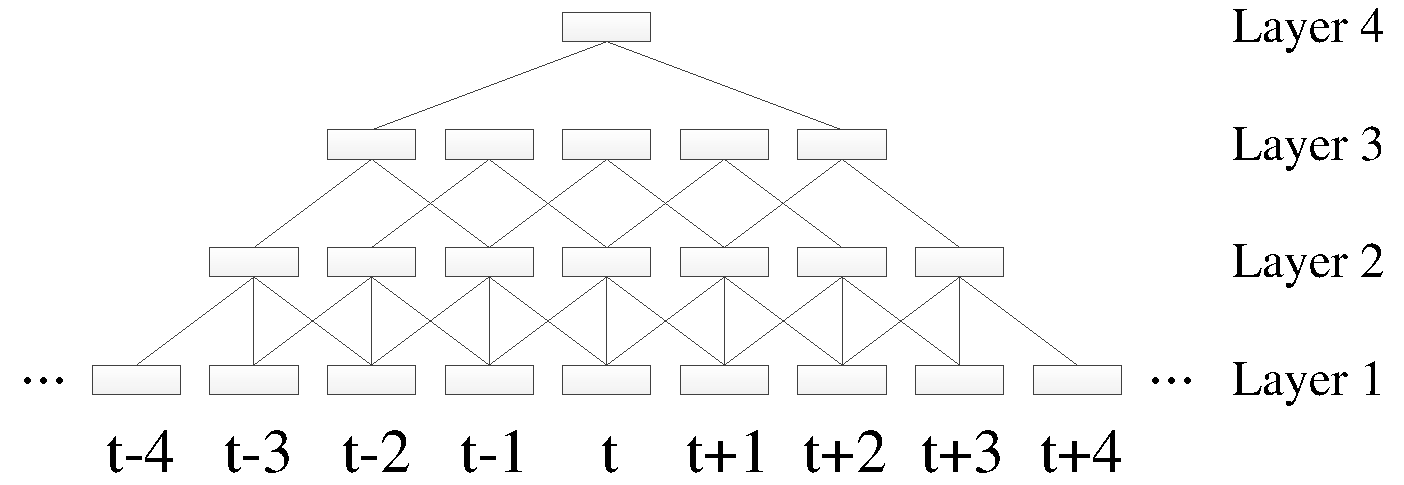
\includegraphics[width = 0.9 \linewidth]{tdnn_emb.pdf}
\caption{A typical TDNN structure}
\label{fig:tdnn}
\end{figure}
In this work, TDNN training algorithm follows greedy layer-wise supervised training with
% parameters updated by
preconditioned stochastic gradient descent (SGD) updates, exponential learning rate schedule and mixing-up, following studies in  \cite{zhang2014improving}.

% Recently it has been found out that a combined TDNN-LSTM AM outperforms BLSTM network in LVCSR \cite{chengexploration}. This work extends to proposing a
% We further extend this and propose a
The proposed TDNN-BLSTM structure combines TDNN and BLSTM by constructing forward and backward pairs of LSTM layers on top of TDNN layers, as illustrated inside dashed box in Figure \ref{fig:SHL-MTDNN-BLSTM}.
% \subsection{Basic layout features}





\subsection{SHL-MTDNN-BLSTM with pre-final layer}
\label{sec:prefinal}
The proposed TDNN-BLSTM applied to SHL-MDNN architecture is denoted as SHL-MTDNN-BLSTM, and illustrated in
% multilingual AM  of SHL-TDNN-BLSTM is illustrated in
Figure \ref{fig:SHL-MTDNN-BLSTM}.
% that the combined TDNN and BLSTM layers are shared between multiple languages, while softmax output layers as well as pre-final layers are language-dependent.
\begin{figure}[tbp]
\centering
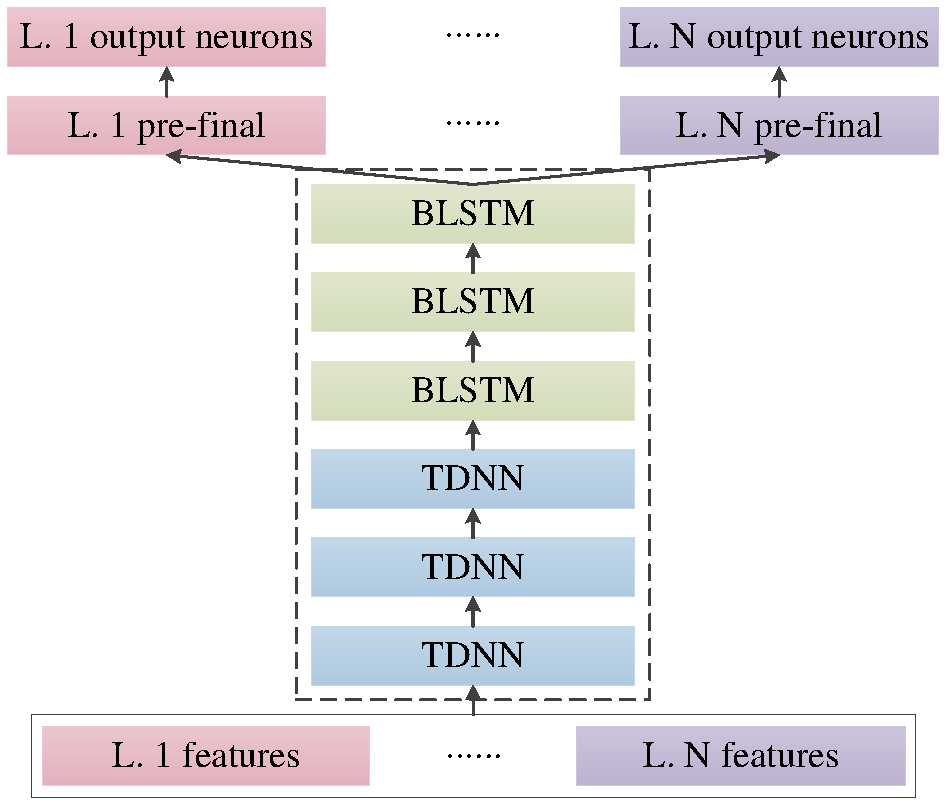
\includegraphics[width= 0.75\linewidth]{SHL_TDNN_BLSTM_PF_font_tnr_emb.pdf}
\caption{The proposed SHL-MTDNN-BLSTM structure}
\label{fig:SHL-MTDNN-BLSTM}
\end{figure}
Different from the widely adopted SHL-MDNN architecture without concerning  any specific hidden layer configuration \cite{Huang2013cross,Zhou2017,karafiat20172016}, in this work,
% and its variants such as SHL-MLSTM \cite{Zhou2017} or SHL-MBLSTM \cite{karafiat20172016},
a language-dependent pre-final hidden layer is proposed to add in under each block-softmax output layer.
% In the conventional SHL-MDNN, universal transformed features are fed directly into block-softmax without any other nonlinear mapping.
We argue that in the conventional SHL-MDNN,  it is unknown to us whether the direct connection between hidden layers and the block-softmax layer is fully capable of modeling the mappings between language-independent universal transformed features and the language-dependent HMM state classification task,
 % is
% CD-HMM state posteriors is
especially while multilingual corpora used for AM training have a diverse range of phonetic and linguistic properties.
The proposed pre-final layer increases nonlinear modeling capability between universal transformed features and language-dependent outputs, thus is expected to facilitate effective cross-lingual knowledge transfer.

% Motivated by this,
% However, few past works has looked into on this.
% In this work, we
% the language-dependent pre-final layer  is added, in order to
% An explicit investigation on the effectiveness of cross-lingual knowledge transferability is made by comparing SHL-MTDNN-BLSTM AM performance with and without the pre-final layer.
 % updated only at back-propagating samples belonging to that language.
 % During network training,
% limit the efficacy of facilitating cross-lingual knowledge transfer
Let $\bm{x_{m}^{i}}$ and $y_{m}^{i}$ denote feature vector and target context-dependent HMM (CD-HMM) state label of the $m$-th training example in the $k$-th minibatch, where $i$ denotes the language identity of $\{\bm{x_{m}^{i}}, y_{m}^{i}\}$.
% $y_{m}^{i}$ denotes the context-dependent HMM state of $\bm{x_{m}^{i}}$.
% where $\{\bm{x_{m}^{i}}, y_{m}^{i}\}$ belongs to the $i$-th language.
The total loss value of the $k$-th minibatch, $L(k)$, is defined as,
\begin{equation}
L(k)=\sum_{m=1}^{M} \omega^{i} l[\theta^{i}(\bm{x_{m}^{i}}), y_{m}^{i}],
\end{equation}
where $M$ is minibatch size, $\omega^{i}$ is task weight of the $i$-th language,
 % normally ranging from $0$ to $1$.
%, representing the importance of model training with data from the $i$-th language.
$\theta^{i}$ denotes nonlinear transform from input to the $i$-th block-softmax output, $l$ is loss function, cross-entropy \cite{vesely2013sequence} adopted in this paper. During network training, CD-HMM state classification errors within a certain language are back-propagated through the corresponding language-dependent pre-final layer and shared TDNN-BLSTM layers, while parameters of block-softmax layers and pre-final layers for the other languages keep unchanged.
% the error caused by $\{\bm{x_{m}^{i}}, y_{m}^{i}\}$ is multiplied by language weight $\omega^{i}$.
% As an instance of multi-task learning (MTL) \cite{caruana1998multitask}, training for each language can be regarded as primary task, while the others will be regarded as secondary tasks.
% Empirically,
% \begin{figure}[htbp]
% \centering
% 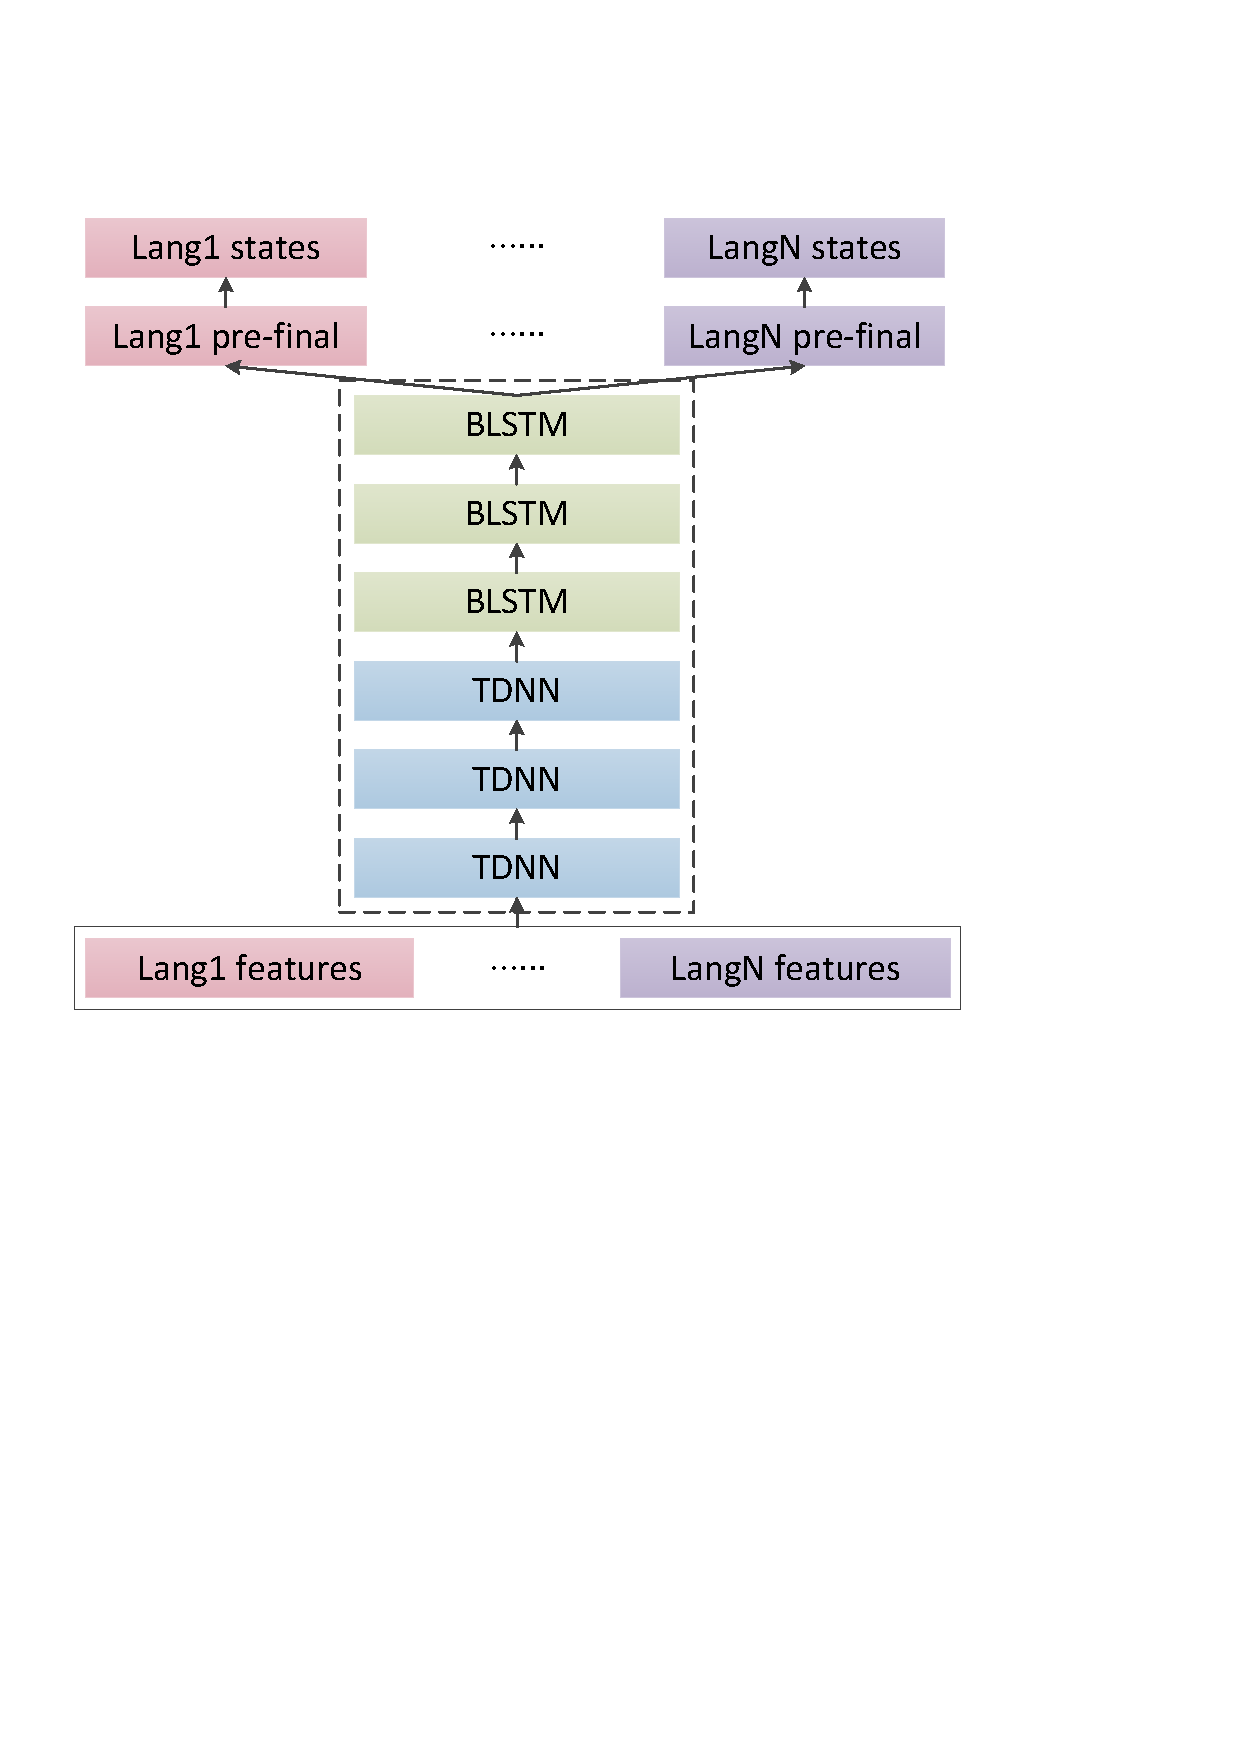
\includegraphics[width= 0.75\linewidth]{SHL_TDNN_BLSTM_PF.pdf}
% \caption{The proposed SHL-MTDNN-BLSTM structure}
% \label{fig:SHL-MTDNN-BLSTM}
% \end{figure}
% During training, parameters of TDNN and BLSTM layers are updated using greedy layer-wise supervised training, preconditioned stochastic gradient descent (SGD) updates, expo

% Different from the widely adopted SHL-MDNN architecture without concerning  any specific hidden layer configuration \cite{Huang2013cross,Zhou2017,karafiat20172016}, in this work,
% % and its variants such as SHL-MLSTM \cite{Zhou2017} or SHL-MBLSTM \cite{karafiat20172016},
% a language-dependent, pre-final hidden layer is proposed to add in before each block-softmax output layer.
% In the conventional SHL-MDNN, universal transformed features are fed directly into block-softmax without any other nonlinear mapping. We argue that whether the block-softmax layer is adequately capable of modeling the mapping between language-independent universal transformed features and language-dependent CD-HMM state posteriors is unknown, especially while multiple languages involved during AM training have a diverse range of phonetic and linguistic properties.
% Motivated by this,
% % However, few past works has looked into on this.
% % In this work, we
% % the language-dependent pre-final layer  is added, in order to
% an explicit investigation on the effectiveness of cross-lingual knowledge transferability is made by comparing SHL-MTDNN-BLSTM AM performance with and without the pre-final layer.

% \subsection{References}

% The reference



\section{Experimental setup}
\label{sec:exp setup}
% This
\subsection{Multilingual corpora}
The datasets used in this work cover three languages: CUSENT in Cantonese (CA), Wall Street Journal (WSJ) in English (EN) and RASC-863 in Mandarin (MA). CUSENT is a read speech corpus  developed by The Chinese University of Hong Kong \cite{LeeLoChingEtAl2002}. There are $20,378$ training utterances from $68$ speakers, and $799$ test utterances from other $8$ speakers. WSJ is a read speech corpus \cite{paul1992design}. The set \emph{si284} is selected as training data, including $37,416$ utterances from $283$ speakers. The set \emph{eval92} is selected as test data, including $333$ utterances from other $8$ speakers. RASC-863 is a read speech corpus containing $89,003$ training utterances from $154$ speakers, and $5,146$ test utterances from other $8$ speakers \cite{li2004rasc863}. Detailed information about the multilingual corpora is listed in Table \ref{tab:datasize_nounit}.

\begin{table}[tbp]
\renewcommand\arraystretch{1}
\centering
\caption{Information about CA, EN and MA corpora}
\resizebox{0.6 \linewidth}{!}{%
\begin{tabular}{rccc}
% \hline
\toprule
Language:  &CA&EN&MA  \\
% \hline
\midrule
Training hours:  & $19.3$ & $81.5$ & $105.3$ \\
Test hours:& $0.6$ & $0.7$ & $5.9$ \\
% \#tied CD-HMM states:& $2462$ & $3431$ & $2386$ \\
% Lexicon size:& $ $ & $ 133K$& $ $ \\
% $\#$ Phonemes: &$43$& $46$&$ 29$& $44$& $38$\\
% \hline
\bottomrule
\end{tabular}%
}
\label{tab:datasize_nounit}
\end{table}

% Basic acoustic units defined for MA are slightly different from those for EN and CA. This is mainly because we hoped to facilitate this research by re-using previously built GMM-HMM systems. In Mandarin, each character is pronounced as a monosyllable, which can be composed of an \emph{Initial} (onset) and a \emph{Final} (rime), according to Hanyu Pinyin System \cite{wiki-no_url:xxx}. \emph{Initials} and \emph{Finals} are used as the basic acoustic units for MA. For EN and CA, phone based acoustic units are used. The detailed information about datasets and basic acoustic units is listed in Table \ref{tab:datasize}.

% % The data sizes are summarized in Table \ref{tab:datasize}.

% \begin{table}[htbp]
% \renewcommand\arraystretch{1}
% \centering
% \caption{Information about CA, EN and MA corpora and basic acoustic units}
% \resizebox{0.75 \linewidth}{!}{%
% \begin{tabular}{rccc}
% % \hline
% \toprule
% Language:  &CA&EN&MA  \\
% % \hline
% \midrule
% Training hours:  & $19.3$ & $81.5$ & $105.3$ \\
% Test hours:& $0.6$ & $0.7$ & $5.9$ \\
% Basic acoustic unit:  & Phone & Phone & Initial-Final \\
% \#basic units (inc. sil):& $33$ & $87$ & $61$ \\
% % \#tied CD-HMM states:& $2462$ & $3431$ & $2386$ \\
% % Lexicon size:& $ $ & $ 133K$& $ $ \\
% % $\#$ Phonemes: &$43$& $46$&$ 29$& $44$& $38$\\
% % \hline
% \bottomrule
% \end{tabular}%
% }
% \label{tab:datasize}
% \end{table}


% \begin{table}[htbp]
% \renewcommand\arraystretch{1}
% \centering
% \caption{TBC}
% \resizebox{0.9 \linewidth}{!}{%
% \begin{tabular}{rccc}
% % \hline
% \toprule
% Language:  &CA&EN&MA  \\
% % \hline
% \midrule
% Basic acoustic unit:  & Phone & Phone & Initial-Final \\
% \#basic units (inc. sil):& $33$ & $87$ & $61$ \\
% \#tied CD-HMM states:& $2462$ & $3431$ & $2386$ \\
% % $\#$ Phonemes: &$43$& $46$&$ 29$& $44$& $38$\\
% % \hline
% \bottomrule
% \end{tabular}%
% }
% \label{tab:phoneinfo}
% \end{table}
\subsection{Feature extraction and alignment generation}

% In this work, the Kaldi speech recognition toolkit is used \cite{povey2011kaldi}.
Mel-frequency cepstral coefficients (MFCCs) without cepstral truncation are used as input features, i.e., $40$-dimensional MFCCs are computed at each time step \cite{povey2014parallel}. MFCCs are spliced with a specific  context size for a certain neural network as will be discussed in Section \ref{sec:baseline}, and further appended with $100$-dimensional i-vectors  to perform instantaneous speaker adaptation. The i-vectors are extracted in an online version,
% An online fashion of i-vector extraction is adopted,
where only frames prior to the current frame, including previous utterances of the same speaker, are used.
% In order to allow the i-vectors to supply the information about any mean offset of the speaker’s data
% These i-vectors have embedded information about the mean offset of speakers' data, so
% Cepstral normalization towards MFCCs is not
% necessary \cite{chengexploration}, thus not
% performed, as speaker information is believed to .
A speed-perturbation method is used to augment training speech data three-fold, with speed factors of $0.9,1.0$ and $1.1$ \cite{ko2015audio}.

% \subsection{***}
% Phone definition, Phone number, CD-HMM state number,
% and probably lexicon size, etc


% To obtain state-level frame alignment piped to neural network training, a
Target labels for both monolingual and multilingual  DNN-HMM hybrid AM training are state level phone alignments. A monolingual CD-GMM-HMM AM for each language is trained beforehand to generate alignments for training data, including original and speed-perturbed speech. These GMM-HMMs are based on $39$-dimensional MFCCs+$\Delta$+$\Delta \Delta$, and processed with linear discriminant analysis (LDA), maximum likelihood linear transform (MLLT) and feature-space maximum likelihood linear regression (fMLLR).
 % estimation to perform feature-level speaker adaptation.
% This GMM-HMM is further used to produce frame alignment of speed-perturbed training data of its corresponding language.
% Syllable error rates (SERs) of GMM-HMM ASR systems for CA and MA are $8.38\%$ and $3.12\%$, WER of GMM-HMM system for EN is $7.97\%$.

It is worth noting that basic acoustic units defined for MA in this work are different from those for EN and CA. This is mainly because we hoped to facilitate this study by re-using previously developed GMM-HMM systems. In Mandarin, each character is pronounced as a monosyllable, which can be composed of an \emph{Initial} (onset) and a \emph{Final} (rime), according to Hanyu Pinyin System \cite{wiki-no_url:xxx}. \emph{Initials} and \emph{Finals} are adopted as the basic acoustic units for MA. For EN and CA, phone based acoustic units are adopted.
\section{Experiments}
\label{sec:exp}
% For Mandarin speech recognition, \textit{Initials} \emph{Initils}and \emph{Finals} are commonly used as the basic units for acoustic modeling \cite{lee2016automatic}.
\subsection{Baseline systems}
\label{sec:baseline}
Baseline systems include monolingual DNN, TDNN, BLSTM and TDNN-BLSTM, all trained with CUSENT training set. There are $300$ training utterances randomly selected as validation data, in order to prevent overfitting. These models are trained on a  cross-entropy criterion. For feature extraction and  acoustic modeling, we use Kaldi toolkit \cite{povey2011kaldi}.
% All these experiments are performed with CA training and test set.

DNN contains $6$ hidden layers with $1024$ neurons per layer, with ReLU activation and batch normalization (ReLU-batchnorm) \cite{ioffe2015batch}. Input MFCCs are spliced with $\pm 5$.
% In other baseline models, TDNN layers are all implemented with ReLU-batchnorm.
TDNN contains $5$ ReLU-batchnorm layers with $1024$ neurons per layer. BLSTM contains $4$ pairs of forward and backward LTSMP layers \cite{sak2014long}, with $1024$-dimensional cells and $256$-dimensional recurrent projections. TDNN-BLSTM is composed of TDNN and forward-backward LSTMP layers, where TDNN layer width is $1024$, LSTMP cell and recurrent projection dimensions are $1024$ and $256$, respectively. The temporal context configurations of TDNN and TDNN-BLSTM are summarized in Table \ref{tab:tdnn_related_config}.
% recurrent projection dimension $130$
% (tell dropout schedule later, at the same time)We found dropout algorithm helpful to
\begin{table}[tbp]
\renewcommand\arraystretch{0.9}
\centering
\caption{Context configurations for TDNN and TDNN-BLSTM}
\resizebox{0.70 \linewidth}{!}{%
\begin{tabular}{c|cc}
% \hline
\toprule
 &TDNN&TDNN-BLSTM \\
\midrule
 Layer  & \multicolumn{2}{c}{Layer context (TDNN) or LSTMP} \\
% \hline
\midrule
1  & $\{-2,-1,0,1,2\}$ & $\{-2,-1,0,1,2\} $\\
2& $\{-1,0,1\}$  & $\{0\}$ \\
3  & $\{-1,0,1\}$ & $\{-1,0,1\}$\\
4 & $\{-3,0,3\}$ &  $\{-1,0,1\}$\\
5 &$\{-6,-3,0\}$& LSTMP-forward\\
6 & $-$ & LSTMP-backward\\
7 & $-$ & LSTMP-forward \\
8 & $-$ & LSTMP-backward \\
9 & $-$ & LSTMP-forward\\
10 & $-$ & LSTMP-backward\\
11& $-$ & LSTMP-forward\\
12& $-$  & LSTMP-backward \\
% 6 & - & &\\
% 7 &   & &\\
% 8 &   & &\\
% 9 &   & &
% \#tied CD-HMM states:& $2462$ & $3431$ & $2386$ \\
% Lexicon size:& $ $ & $ 133K$& $ $ \\
% $\#$ Phonemes: &$43$& $46$&$ 29$& $44$& $38$\\
% \hline
\bottomrule
\end{tabular}%
}
\label{tab:tdnn_related_config}
\end{table}
For DNN and TDNN, the number of training epochs is $3$, learning rate starts from $1.5\times 10^{-2}$ to $1.5\times 10^{-3}$ with exponential decay, minibatch size is $256$. For BLSTM and TDNN-BLSTM models, the number of training epochs is $6$, minibatch size is $128$, learning rate starts from $3\times 10^{-3}$ to $3\times 10^{-4}$, also with exponential decay.
A dropout method is adopted during network training,
% all the baseline models
in order to improve generalization \cite{chengexploration}. Dropout probability $p(n)$ with respect to training iterations $n$ is  piece-wise linear, as described below,
\begin{equation}
    p(n)=
   \begin{cases}
   0.2 \times \frac{n}{N}, &\mbox{$0 \le n \le \frac{N}{2}$}\\
   0.2 \times (1-\frac{n}{N}), &\mbox{$\frac{N}{2} \le n \le N$}
   \end{cases}
  \end{equation}
where $N$ is the number of iterations. Note that the choices of training hyperparameters and TDNN temporal contexts basically follow Kaldi default settings.
%illustrated in Figure \ref{fig:dropout}. The Kaldi \emph{nnet3} recipe is used to train all the neural network acoustic models \cite{povey2011kaldi}.
% For the sake of convenience,
%\begin{figure}[htbp]
%\centering
%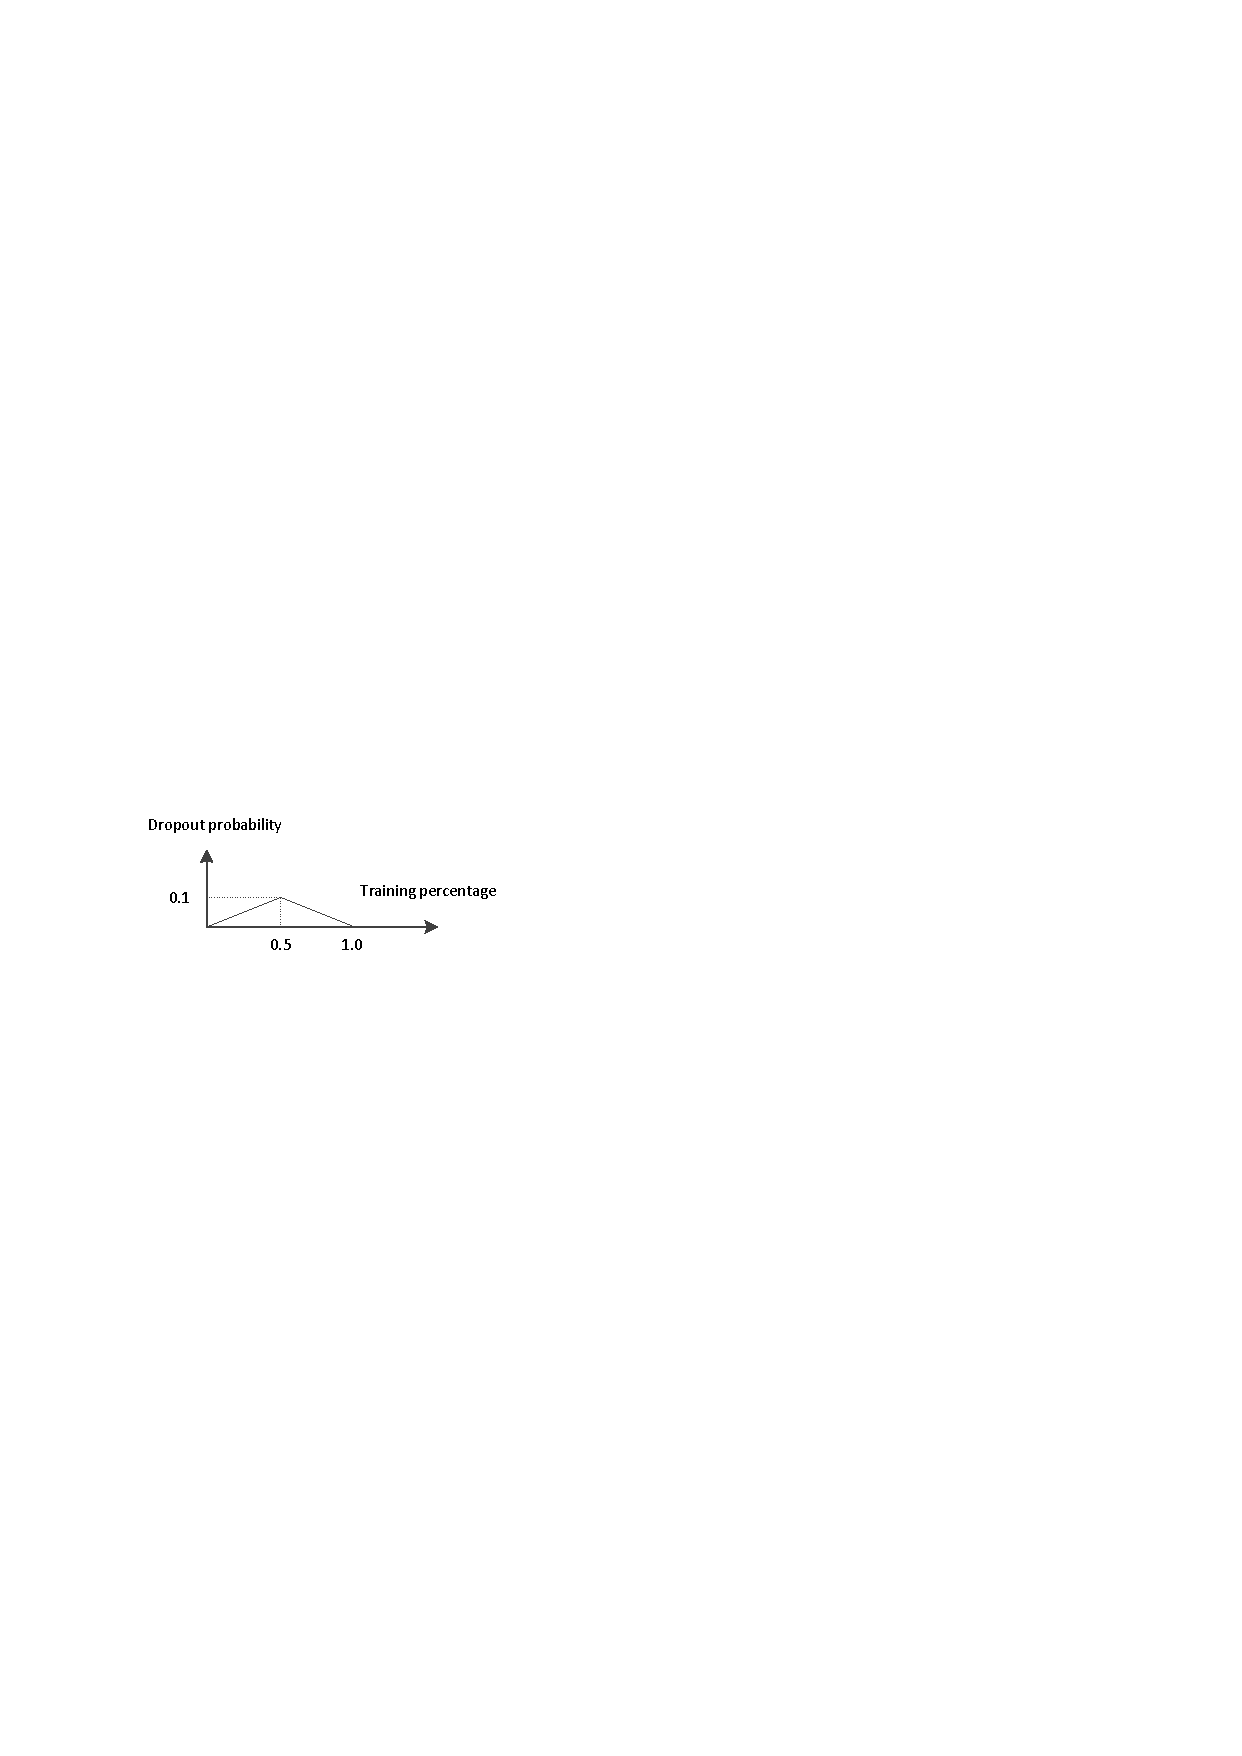
\includegraphics[width= 0.7\linewidth]{Dropout_prob.pdf}
%\caption{Dropout probability w.r.t training epochs}
%\label{fig:dropout}
%\end{figure}

% The dropout schedule is set as $'0, 0@0.2, 0.1@0.5, 0'$, which means the dropout probability varies through training epochs. From beginning to $20\%$ of training process, dropout probability is $0$.

\subsection{Results and analyses}
For multilingual acoustic modeling, DNN, TDNN, BLSTM and TDNN-BLSTM  are implemented in the SHL-MDNN architecture. Layer configurations are set the same as in baseline monolingual models, plus the language-dependent pre-final layer as proposed in Section \ref{sec:prefinal}. The pre-final layer is implemented by ReLU-renorm in Kaldi \emph{nnet3} recipe, with $1024$ neurons. Learning rate and minibatch sizes for multilingual AM training are consistent with corresponding baseline model settings. The number of training epochs for DNN and TDNN is $2$, BLSTM and TDNN-BLSTM is $4$. The dropout probability is constant $0.1$ for forward-backward LSTMP layers, and $0$ for DNN or TDNN layers, as we find this to be optimal in multilingual acoustic modeling.
EN and/or MA are merged with CA to form various multilingual training corpora. Similar to baseline model training, for each corpus, there are $300$ training utterances randomly selected as validation set. Syllable error rates (SERs) of CA test set is chosen for evaluation. A syllable trigram language model trained with transcriptions of CA training data is used during decoding, using SRILM toolkit \cite{Stolcke02srilm--}. SERs of baseline and multilingual systems are listed in Table \ref{tab:mono_vs_multi}.
\begin{table}[tbp]
\renewcommand\arraystretch{0.85}
\centering
\caption{SERs of baseline and multilingual systems with optimized language weights}
\resizebox{ 0.9\linewidth}{!}{%
\begin{tabular}{ccc|c}
% \hline
\toprule
Model & Training language(s) & \#parameters & SER\% \\

 % Model&DNN&TDNN&BLSTM& TD-LS & TD-BLS  \\
\midrule
DNN & CA & $8.3$M & $7.37$ \\
TDNN & CA & $15.4$M& $6.34$\\
BLSTM & CA & $42.8$M & $6.67$\\
% TDNN-LSTM & CA &$?$M &$6.51$\\
TDNN-BLSTM & CA &$56.4$M &$6.31$\\
 \midrule
DNN & CA, EN:$0.7,0.3$ & $14.2$M & $6.54$ \\
TDNN & CA, EN:$0.6,0.4$ & $21.1$M& $5.99$\\
BLSTM & CA, EN:$0.7,0.3$ & $48.5$M& $6.45$\\
% TDNN-LSTM & CA,EN:$0.7,0.3$ &$? $M &$ ?$\\
TDNN-BLSTM & CA, EN:$0.8,0.2$ &$62.0$M &$5.79$\\
TDNN & CA, MA:$0.8,0.2$ &$20.1$M &$5.93$\\
TDNN-BLSTM & CA, MA:$0.9,0.1$ &$60.9$M &$6.21$\\

TDNN & CA, EN, MA:$0.65,0.25,0.1$ & $24.6$M& $5.75$\\
TDNN-BLSTM & CA, EN, MA:$0.65,0.2,0.15$ &$65.5$M &$\bm{5.50}$\\

% \hline

% \midrule

% 6 & - & &\\
% 7 &   & &\\
% 8 &   & &\\
% 9 &   & &
% \#tied CD-HMM states:& $2462$ & $3431$ & $2386$ \\
% Lexicon size:& $ $ & $ 133K$& $ $ \\
% $\#$ Phonemes: &$43$& $46$&$ 29$& $44$& $38$\\
% \hline
\bottomrule
\end{tabular}%
}
\label{tab:mono_vs_multi}
\end{table}
\begin{figure}[tbp]
\centering
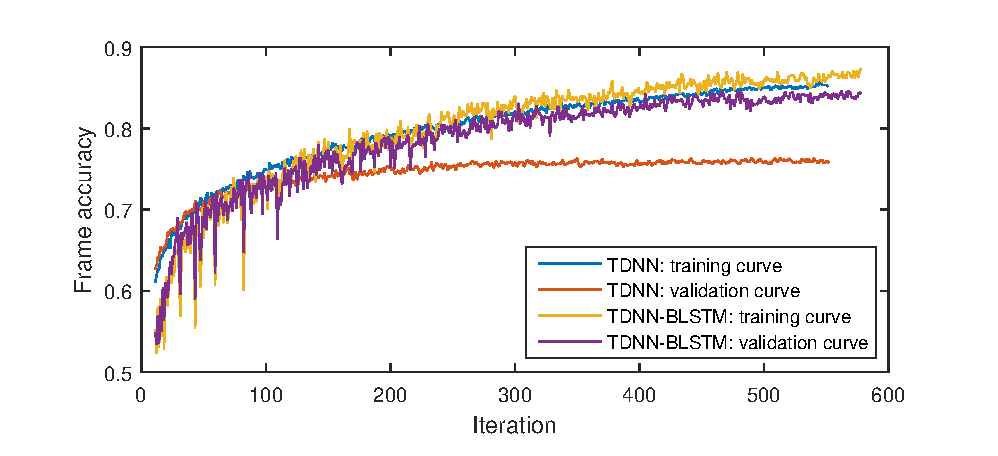
\includegraphics[width= 0.97\linewidth]{curve.eps}
\caption{Frame accuracy curves during TDNN and TDNN-BLSTM training with merged CA, EN and MA corpora}
\label{fig:curve}
\end{figure}
%\begin{figure}[htbp]
%\centering
%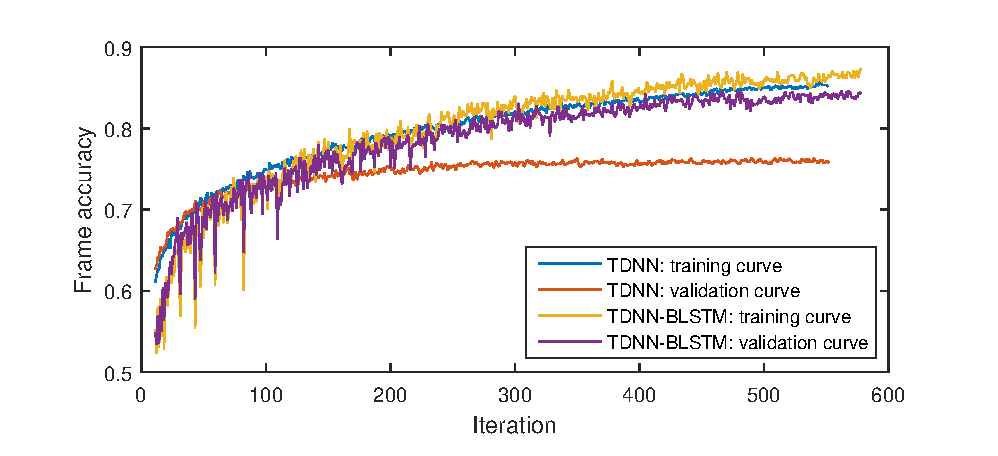
\includegraphics[width= \linewidth]{curve.eps}
%\caption{Frame accuracy of training and validation data during TDNN and TDNN-BLSTM training using CA+EN+MA}
%\label{fig:curve}
%\end{figure}
Note that in this Table, SERs of multilingual systems with only the optimized language weight are listed. The corresponding language weight is specified right after training language identities. Figure \ref{fig:curve} compares frame accuracy curves during training of TDNN and TDNN-BLSTM, with merged CA, EN and MA corpora.
% \begin{figure}[tbp]
% \centering
% 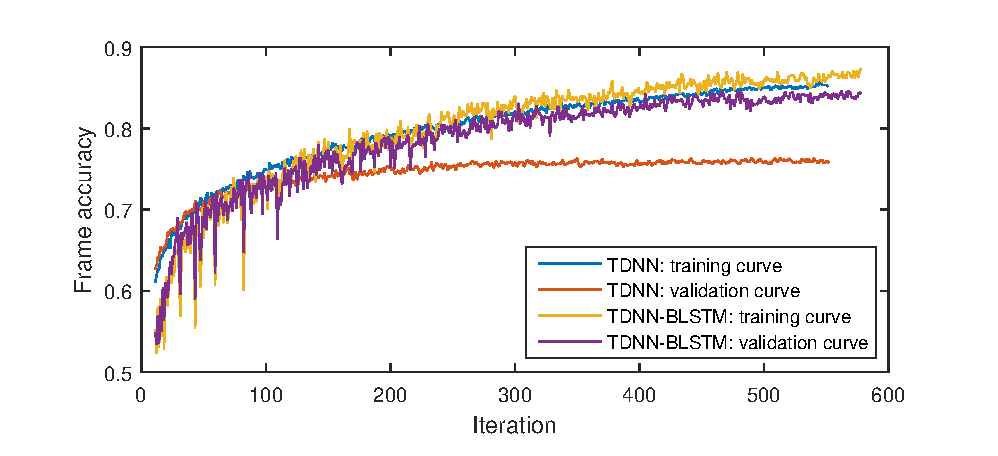
\includegraphics[width= \linewidth]{curve.eps}
% \caption{Frame accuracy curves during TDNN and TDNN-BLSTM training with merged CA, EN and MA corpora}
% \label{fig:curve}
% \end{figure}
From Table \ref{tab:mono_vs_multi} and Figure \ref{fig:curve}, the following observations are made:
% \begin{itemize}

(1) Multilingual models of DNN, TDNN, BLSTM and TDNN-BLSTM using merged CA and EN corpora outperform their monolingually trained counterparts, with relative improvements ranging from $3.3\%$ to $11.3\%$. This result is generally in line with past works \cite{Huang2013cross,Zhou2017}.

(2) TDNN-BLSTM achieves the best Cantonese ASR performance among all neural network structures in both monolingual and multilingual training, with SERs $6.31\%$ and $5.50\%$, respectively. Moreover,
% validation data frame accuracy curve during multilingual TDNN-BLSTM training converges to a significantly higher value than that of TDNN. B
by observing frame accuracy curves, the generalization capability of the trained TDNN-BLSTM is stronger than TDNN.
% trained TDNN-BLSTM shows stronger generalization capability than TDNN.

%, except for a slight inferior to TDNN when using CA and MA datasets.
% The combined network, TDNN-BLSTM, has shown advantage over TDNN and BLSTM models in both monolingual and multilingual training strategies.
% By merging CA, EN and MA, TDNN-BLSTM model can yield a further gain to $5.59\%$, while TDNN model ($5.90\% \rightarrow 5.88\%$) does not show significant improvement.
(3) Compared with TDNN-BLSTM and TDNN,
 % trained with monolingual CA corpus and multilingual corpora,
it can be observed that the achieved  SER reduction from monolingual (CA) training to multilingual training is larger for TDNN-BLSTM than for TDNN.
% resulting from including multilingual training sets is larger for TDNN-BLSTM than for TDNN.
% TDNN-BLSTM achieves greater SER reduction  than TDNN in multilingual training than in monolingual case.
%the advantage of TDNN-BLSTM over TDNN increases when training languages increase.
This
% not only demonstrates our assumption that TDNN-BLSTM could bring improved ASR performance in multilingual acoustic model training, in comparison with other commonly adopted neural network structures, but also
shows the stronger modeling capability of TDNN-BLSTM as compared to TDNN, especially in the context of multilingual acoustic modeling. On the other hand, the model size of TDNN-BLSTM is significantly larger than TDNN, hence much more computational resources are required.
% requiring much more computational and memory resources.
% especially with larger variety of training languages and data size.
%\item[(d)] When trained with merged CA and MA datasets, both TDNN-BLSTM and TDNN perform less well as compared to those trained by CA and EN datasets, although they both outperform monolingual training baseline. As training data quantity of MA is larger than EN by about $29\%$, there is no reason to regard this issue as a data size problem. We suppose it is due to the different definition of basic acoustic units for MA, \emph{Initial-Final}. Further research is needed to investigate more on the influence caused by different acoustic unit definitions on multilingual neural network acoustic modeling.
% \end{itemize}
% \subsection{}

\subsection{The effectiveness of the pre-final layer}
The effectiveness of language-dependent pre-final layer is of great interest to us. We report our experimental results based on SHL-MTDNN-BLSTM model with the optional pre-final layer. Various training language identities are adopted to train SHL-MTDNN-BLSTM, as illustrated in Table \ref{tab:PF_vs_no_PF}. CA test set is chosen for evaluation. Experimental results are summarized as in Table \ref{tab:PF_vs_no_PF}. Note that language weights listed in this Table are all optimized ones.
%\begin{table}[htbp]
%\renewcommand\arraystretch{1}
%\centering
%\caption{SERs of multilingual TDNN and TDNN-BLSTM with or without pre-final layers }
%\resizebox{0.85 \linewidth}{!}{%
%\begin{tabular}{c|cc|cc}
%% \hline
%\toprule
%% \multirow{2}{*}{Language weight}  & \multicolumn{2}{c|}{TDNN} & \multicolumn{2}{c}{TDNN-BLSTM} \\
%% & W/ PF & W/o PF & W/ PF & W/o PF \\
%
%Language weight & \multicolumn{2}{c|}{TDNN} & \multicolumn{2}{c}{TDNN-BLSTM} \\
%CA, EN, MA &  W/ PF & W/o PF & W/ PF & W/o PF \\
% % Model&DNN&TDNN&BLSTM& TD-LS & TD-BLS  \\
%\midrule
%
%$0.7,0.2,0.1$ & $5.84$ & $?$ & $5.59$ & $5.54$ \\
%$0.8,0.2,0$ & $6.07$ & $?$ & $5.79$ & $6.00$ \\
%$0.8,0,0.2$ & $5.93$ & $?$ & $6.11$ & $?$ \\
%
%% \hline
%
%% \midrule
%
%% 6 & - & &\\
%% 7 &   & &\\
%% 8 &   & &\\
%% 9 &   & &
%% \#tied CD-HMM states:& $2462$ & $3431$ & $2386$ \\
%% Lexicon size:& $ $ & $ 133K$& $ $ \\
%% $\#$ Phonemes: &$43$& $46$&$ 29$& $44$& $38$\\
%% \hline
%\bottomrule
%\end{tabular}%
%}
%\label{tab:PF_vs_no_PF}
%\end{table}
\begin{table}[tbp]
\renewcommand\arraystretch{0.9}
\centering
\caption{SERs of SHL-MTDNN-BLSTM with/without pre-final layer }
\resizebox{0.83 \linewidth}{!}{%
\begin{tabular}{c|cc}
% \hline
\toprule
% \multirow{2}{*}{Language weight}  & \multicolumn{2}{c|}{TDNN} & \multicolumn{2}{c}{TDNN-BLSTM} \\
% & W/ PF & W/o PF & W/ PF & W/o PF \\

Training languages: Weights   &     With pre-final & Without pre-final \\
% \midrule
% &   \\
 % Model&DNN&TDNN&BLSTM& TD-LS & TD-BLS  \\
\midrule

CA, EN, MA: $0.65,0.2,0.15$ &  $5.50$ & $5.52$ \\
CA, EN: $0.8,0.2$ &  $5.79$ & $6.00$ \\
CA, MA: $0.9,0.1$ &  $6.21$ & $6.54$ \\

% \hline

% \midrule

% 6 & - & &\\
% 7 &   & &\\
% 8 &   & &\\
% 9 &   & &
% \#tied CD-HMM states:& $2462$ & $3431$ & $2386$ \\
% Lexicon size:& $ $ & $ 133K$& $ $ \\
% $\#$ Phonemes: &$43$& $46$&$ 29$& $44$& $38$\\
% \hline
\bottomrule
\end{tabular}%
}
\label{tab:PF_vs_no_PF}
\end{table}

As can be seen from  Table \ref{tab:PF_vs_no_PF},
%except for TDNN-BLSTM trained by CA, EN and MA datasets with $0.7,0.2,0.1$, which approximately performs the same by adding/removing language-dependent pre-final layers,
 SHL-MTDNN-BLSTM with the pre-final layer brings moderate while consistent  ASR performance improvements in various multilingual corpora settings,
 % lower or comparable SERs on
 % Cantonese ASR task,
 in comparison with those without the pre-final layer. This indicates that
% for neural network acoustic model structures with relatively less strong modeling capacities,
 the conventional SHL-MDNN architecture
 % , where the universal transformed features generated by shared hidden layers directly pass to block-softmax layers without any language-specific nonlinear transform,
 may be suboptimal in modeling the mappings between language-independent features and language-dependent outputs.
 % CD-HMM state posteriors of a specific language.
 The pre-final layer could alleviate this problem and facilitate effective cross-lingual knowledge transfer through increasing nonlinear modeling capability between shared hidden layers and network outputs.
 % provides additional nonlinearity to language-dependent structures in SHL-MDNN, hence
 % is able to increase nonlinear modeling capability for mapping between language-independent features and language-dependent outputs,
  % and brings SER reduction in multilingually trained Cantonese ASR systems,
 % and bimproves  cross-lingual knowledge transferability.

 % Future works may include detailed investigation on whether and how the effectiveness of our proposed pre-final layer is influenced by diverse linguistic dissimilarities within multilingual corpora. More studies are also needed to measure the effect of mismatched basic acoustic unit definitions on multilingual acoustic modeling.
 % the influence of linguistically similar/dissimilar languages for multilingual acoustic modeling with the proposed language-dependent pre-final layer.
 %It can be seen that the pre-final layer takes effect on all CA+EN, CA+MA and CA+EN+MA multilingual dataset configuration. This naturally raises concern, as
 % as the bridge to connect language-independent features and language-specific acoustic-phonetic properties.
 % Intuitively, SHL-MDNN trained by using multiple languages with similar linguistic characteristics to the target language may be less affected by the pre-final layer configuration, it's believed that acoustic-phonetic properties of these languages are assumed to be close to each other. This may be investigated in our future research.
% \subsection{Results with different language weights}
% \section{Experimental results}
\section{Conclusions and future works}
\label{sec:concl}
This paper presents a study on improving multilingual acoustic modeling for ASR, in the context of SHL-MDNN AM architecture. Two research aspects are investigated. Firstly, the shared hidden layer configuration is replaced  with the more advanced, TDNN-BLSTM structure. Secondly, the SHL-MDNN architecture is modified by adding the proposed language-dependent pre-final layer under each block-softmax output layer, with the goal of improving  cross-lingual knowledge transferability.
 % the comparison of multilingual acoustic modeling for ASR, using different neural networks such as DNN, TDNN, BLSTM, and the proposed TDNN-BLSTM, in which forward-backward LSTM layers are constructed on top of TDNN layers.
% Different from the widely adopted multilingual SHL-MDNN architecture,
% Moreover, a language-dependent pre-final layer is added in under each block-softmax output layer.
% It is expected that the pre-final layer could increase nonlinear modeling capability for mapping between universal transformed features and language-specific outputs.
Experiments are carried out with multilingual corpora covering Cantonese, English and Mandarin. A Cantonese ASR task is selected for evaluation.
% read speech corpora including three languages, i.e., CUSENT (Cantonese), WSJ (English) and RASC-863 (Mandarin). CUSENT test set is selected for evaluation.
Experimental results show that multilingual AMs consistently outperform their monolingual counterparts. Multilingual TDNN-BLSTM model trained with the three corpora achieves the best ASR performance, meanwhile preserving strong generalization capability.
 % compared with DNN, TDNN and BLSTM.
 The language-dependent pre-final layer could bring moderate while consistent improvements in various multilingual training corpora settings, thus demonstrates its effectiveness in improving
 % , as compared to the structure without the pre-final layer.
 % It is expected that the language-dependent pre-final layer leads to improved
 cross-lingual knowledge transferability.
  % by increasing nonlinear modeling capability for mapping between universal transformed features and language-specific outputs.

% shows advantage over conventional multilingual .
% Authors must proofread their PDF file prior to submission to ensure it is correct. Authors should not rely on proofreading the Word file. Please proofread the PDF file before it is submitted.



% The ISCA Board would like to thank the organizing committees of the past INTERSPEECH conferences for their help and for kindly providing the template files.
Future works include detailed investigation on whether and how the effectiveness of our proposed pre-final layer is influenced by diverse linguistic dissimilarities within different groups of multilingual corpora, and the
% As there is a mismatch in the definition of basic acoustic units among training languages, m
% More studies are needed to measure the
effect of basic acoustic unit definition mismatch on multilingual acoustic modeling.


\section{Acknowledgements}
We thank Yuzhong Wu for providing processed RASC-863 dataset.
This research is partially supported by a GRF project grant (Ref: CUHK 14227216) from Hong Kong Research Grants Council.

\bibliographystyle{IEEEtran}

\bibliography{mybib}



\end{document}
